%%%%%%%%%%%%%%%%%%%%%%%%%%%%%%%%%%%%%%%%%%%%%%%%%%%%%%%%%%%%%%%%%%%%%%%%

%%% LaTeX Template for AAMAS-2025 (based on sample-sigconf.tex)
%%% Prepared by the AAMAS-2025 Program Chairs based on the version from AAMAS-2025. 

%%%%%%%%%%%%%%%%%%%%%%%%%%%%%%%%%%%%%%%%%%%%%%%%%%%%%%%%%%%%%%%%%%%%%%%%

%%% Start your document with the \documentclass command.


%%% == IMPORTANT ==
%%% Use the first variant below for the final paper (including auithor information).
%%% Use the second variant below to anonymize your submission (no authoir information shown).
%%% For further information on anonymity and double-blind reviewing, 
%%% please consult the call for paper information
%%% https://aamas2025.org/index.php/conference/calls/submission-instructions-main-technical-track/

%%%% For anonymized submission, use this
\documentclass[sigconf,nonacm]{aamas}

%%%% For camera-ready, use this
% \documentclass[sigconf]{aamas} 


%%% Load required packages here (note that many are included already).

\usepackage{balance} % for balancing columns on the final page
\usepackage{multirow}

%%%%%%%%%%%%%%%%%%%%%%%%%%%%%%%%%%%%%%%%%%%%%%%%%%%%%%%%%%%%%%%%%%%%%%%%

%%% AAMAS-2025 copyright block (do not change!)

% \setcopyright{ifaamas}
% \acmConference[AAMAS '25]{Proc.\@ of the 24th International Conference
% on Autonomous Agents and Multiagent Systems (AAMAS 2025)}{May 19 -- 23, 2025}
% {Detroit, Michigan, USA}{A.~El~Fallah~Seghrouchni, Y.~Vorobeychik, S.~Das, A.~Nowe (eds.)}
% \copyrightyear{2025}
% \acmYear{2025}
% \acmDOI{}
% \acmPrice{}
% \acmISBN{}


%%%%%%%%%%%%%%%%%%%%%%%%%%%%%%%%%%%%%%%%%%%%%%%%%%%%%%%%%%%%%%%%%%%%%%%%

%%% == IMPORTANT ==
%%% Use this command to specify your submission number.
%%% In anonymous mode, it will be printed on the first page.

% \acmSubmissionID{51}

%%% Use this command to specify the title of your paper.

\title{Perspectives for Direct Interpretability in Multi-Agent Deep Reinforcement Learning}

%%% Provide names, affiliations, and email addresses for all authors.

\author{Yoann Poupart}
\affiliation{
  \institution{LIP6, Sorbonne University}
  \city{Paris}
  \country{France}
  }
\email{yoann.poupart@lip6.fr}

\author{Aurélie Beynier }
\affiliation{
  \institution{LIP6, Sorbonne University}
  \city{Paris}
  \country{France}
}
\email{aurelie.beynier@lip6.fr}

\author{Nicolas Maudet }
\affiliation{
  \institution{LIP6, Sorbonne University}
  \city{Paris}
  \country{France}
}
\email{nicolas.maudet@lip6.fr}

%%% Use this environment to specify a short abstract for your paper.

\begin{abstract}
Multi-Agent Deep Reinforcement Learning (MADRL) was proven efficient in solving complex problems in robotics or games, yet most of the trained models are hard to interpret. While learning intrinsically interpretable models remains a prominent approach, its scalability and flexibility are limited in handling complex tasks or multi-agent dynamics. This paper advocates for direct interpretability, generating post hoc explanations directly from trained models, as a versatile and scalable alternative, offering insights into agents' behaviour, emergent phenomena, and biases without altering models' architectures. We explore modern methods, including relevance backpropagation, knowledge edition, model steering, activation patching, sparse autoencoders and circuit discovery, to highlight their applicability to single-agent, multi-agent, and training process challenges. By addressing MADRL interpretability, we propose directions aiming to advance active topics such as team identification, swarm coordination and sample efficiency.
\end{abstract}

%%% The code below was generated by the tool at http://dl.acm.org/ccs.cfm.
%%% Please replace this example with code appropriate for your own paper.


%%% Use this command to specify a few keywords describing your work.
%%% Keywords should be separated by commas.

\keywords{Interpretability, Multi-Agent Systems, Reinforcement Learning, Deep Neural Networks}

%%%%%%%%%%%%%%%%%%%%%%%%%%%%%%%%%%%%%%%%%%%%%%%%%%%%%%%%%%%%%%%%%%%%%%%%

%%% Include any author-defined commands here.
         
\newcommand{\BibTeX}{\rm B\kern-.05em{\sc i\kern-.025em b}\kern-.08em\TeX}


\usepackage{xcolor}
\usepackage{ulem}

% \newcommand{\imenea}[1]{\textcolor{red}{\textbf{#1}}}
% \newcommand{\imeneq}[1]{\textcolor{blue}{\textbf{Imene: #1}}}
% \newcommand{\imener}[1]{\textcolor{purple}{\textbf{\sout{#1}}}}
% \newcommand{\yoannr}[1]{\textcolor{green}{\textbf{#1}}}
% \newcommand{\added}[1]{\textcolor{red}{\textbf{#1}}}

%%%%%%%%%%%%%%%%%%%%%%%%%%%%%%%%%%%%%%%%%%%%%%%%%%%%%%%%%%%%%%%%%%%%%%%%

\begin{document}

%%% The following commands remove the headers in your paper. For final 
%%% papers, these will be inserted during the pagination process.

\pagestyle{fancy}
\fancyhead{}

%%% The next command prints the information defined in the preamble.

\maketitle 

%%%%%%%%%%%%%%%%%%%%%%%%%%%%%%%%%%%%%%%%%%%%%%%%%%%%%%%%%%%%%%%%%%%%%%%%


% \begin{figure*}[htb!]
% \noindent\fbox{
% \parbox{.98\textwidth}{
% \color{teal}{
% I have some texts along with their corresponding scores. The texts are arranged in ascending order based on their scores, where higher scores indicate better quality.

% }

% \vspace{1em}
% \color{darkgreen}{
% text:

% The following are multiple-choice questions (with answers) about professional medicine. Please choose the correct answer from 'A', 'B', 'C' or 'D'.

% score:

% 61

% \vspace{1em}

% text:

% Below is a multiple-choice question related to professional medicine. Review the question carefully and select the correct answer from the options 'A', 'B', 'C', or 'D'. 

% score:

% 63

% \vspace{1em}
% (… more instructions and scores …)
% \vspace{1em}
% }

% \color{teal}{
% The following exemplars show how to apply your text: you replace <INS> in each input with your text, then read the input and give an output. We say your output is wrong if it is different from the given output, and we say your output is correct if they are the same.
% }
% \color{brown}{
% \vspace{1em}

% input:

% Q: A 13-month-old child is brought to the emergency department because of urticaria, swelling of the lips, and difficulty breathing immediately after eating an egg. A potential risk for hypersensitivity reaction is posed by vaccination against which of the following illnesses?
% A: Hepatitis
% B: Influenza
% C: Pertussis
% D: Poliomyelitis

% A: <INS>

% output:

% B

% \vspace{1em}
% (… more exemplars …)
% \vspace{1em}
% }

% \color{teal}{
% Write your new text that is different from the old ones and has a high score. Write the text in square brackets.}
% }
% }
% \caption{Illustration of prompt optimization using instruction-tuned Palm2 Text-bison in MMLU professional medicine. The generated answer is inserted at the beginning of ``A:'' in the scorer LLM output, marked by <INS>. The \textcolor{darkgreen}{green} text shows case-score pairs, the \textcolor{brown}{brown} text outlines the optimization task and output format, and the \textcolor{teal}{teal} text provides reference-instructions.
% }
% \label{fig:reference_prompt_example}
% \end{figure*}

% \begin{figure*}[htb!]
% \centering
% \begin{tcolorbox}[width=0.98\textwidth, colframe=black, boxrule=0.5pt, arc=0mm, colback=white,
%   left=4pt, right=4pt, top=4pt, bottom=4pt]
% \small 

% {\color{teal}
% I have some prompts along with their corresponding scores. The prompts are arranged in ascending order based on their scores, where higher scores indicate better quality.
% }

% \medskip

% {\color{darkgreen}
% \textbf{Prompt 1:}

% The following are multiple-choice questions about professional medicine. Please choose the correct answer from 'A', 'B', 'C', or 'D'.

% \textbf{Score:} 61

% \medskip

% \textbf{Prompt 2:}

% Below is a multiple-choice question related to professional medicine. Review the question carefully and select the correct answer from the options 'A', 'B', 'C', or 'D'.

% \textbf{Score:} 63

% \medskip

% \textbf{Prompt 3:}

% You will be presented with a professional medical multiple-choice question. Please read carefully and choose the correct option from 'A', 'B', 'C', or 'D'.

% \textbf{Score:} 65

% \medskip

% (… more prompts and scores …)
% }

% \medskip

% {\color{teal}
% The following exemplars show how to apply your prompt: you replace \texttt{<INS>} in each input with your prompt, then read the input and provide the correct answer. We say your output is correct if it matches the given output, and incorrect if it does not.

% Please write a new prompt that is different from the previous ones and aims to achieve a higher score. Write your new prompt in square brackets [ ].
% }

% \medskip

% {\color{brown}
% \textbf{Input:}

% \textbf{A:} \texttt{<INS>}

% Q: A 13-month-old child is brought to the emergency department because of urticaria, swelling of the lips, and difficulty breathing immediately after eating an egg. A potential risk for hypersensitivity reaction is posed by vaccination against which of the following illnesses?
% A: Hepatitis
% B: Influenza
% C: Pertussis
% D: Poliomyelitis



% \medskip

% \textbf{Expected Output:}

% B

% \medskip

% (… more examples …)
% }
% \end{tcolorbox}
% \caption{An illustration of the reference-prompt used in the POI method. The \textcolor{darkgreen}{green} text shows previously generated prompts and their scores, the \textcolor{brown}{brown} text provides example inputs and expected outputs for the optimization task, and the \textcolor{teal}{teal} text contains instructions for generating a new prompt.
% }
% \label{fig:reference_prompt_example}
% \end{figure*}


\begin{figure*}[t] \noindent\fbox{ \parbox{\textwidth}{ \color{teal}{ I have some instructions along with their corresponding scores. The instructions are arranged in ascending order based on their scores, where higher scores indicate better quality. }

\vspace{1em} \color{darkgreen}{ text:

The following are multiple choice questions (with answers) about professional medicine. Please choose the correct answer from "A", "B", "C", or "D".

score:

61

\vspace{1em}

text:

Below is a multiple-choice question related to professional medicine. Review the question carefully and select the correct answer from the options "A", "B", "C", or "D".

score:

63

\vspace{1em} (… more instructions and scores …) \vspace{1em} }

\color{teal}{ The following examples demonstrate how to apply your instruction: you replace <INS> in each input with your instruction, then read the input and provide an output. Your output is considered correct if it matches the given output. }

\color{brown}{ \vspace{1em}

input:

Q: A 13-month-old child is brought to the emergency department because of urticaria, swelling of the lips, and difficulty breathing immediately after eating an egg. A potential risk for hypersensitivity reaction is posed by vaccination against which of the following illnesses?
A: Hepatitis
B: Influenza
C: Pertussis
D: Poliomyelitis

A: <INS>

output:

B

\vspace{1em} (… more examples …) \vspace{1em} }

\color{teal}{ Please write a new instruction that is different from the ones given and aims for the highest possible score. Write your instruction in square brackets. } } } \caption{\small An example of the meta-prompt for prompt optimization using instruction-tuned models on the MMLU professional medicine dataset. The generated instruction is inserted at the position marked by <INS> in the input. The \textcolor{darkgreen}{dark green} text displays instruction-score pairs; the \textcolor{brown}{brown} text provides examples of how to apply the instruction; the \textcolor{teal}{teal} text contains the meta-instructions.} \label{fig
} \end{figure*}


% \begin{figure*}[htb!]
% \centering
% \begin{tcolorbox}[width=0.98\textwidth, colframe=black, boxrule=0.5pt, arc=0mm, colback=white,
%   left=4pt, right=4pt, top=4pt, bottom=4pt]
% \small % 使用较小的字体大小
% {\color{teal}
% I have some texts along with their corresponding scores. The texts are arranged in ascending order based on their scores, where higher scores indicate better quality.
% }

% \medskip

% {\color{darkgreen}
% \textbf{prompt:} The following are multiple-choice questions (with answers) about professional medicine. Please choose the correct answer from 'A', 'B', 'C' or 'D'.

% \textbf{score:} 61

% \medskip

% \textbf{prompt:} Below is a multiple-choice question related to professional medicine. Review the question carefully and select the correct answer from the options 'A', 'B', 'C', or 'D'.

% \textbf{score:} 63

% \medskip

% (… more instructions and scores …)
% }

% \medskip

% {\color{teal}
% The following exemplars show how to apply your text: you replace \texttt{<INS>} in each input with your text, then read the input and give an output. We say your output is wrong if it is different from the given output, and we say your output is correct if they are the same.
% }

% \medskip

% {\color{brown}
% \textbf{Input:}

% Q: A 13-month-old child is brought to the emergency department because of urticaria, swelling of the lips, and difficulty breathing immediately after eating an egg. A potential risk for hypersensitivity reaction is posed by vaccination against which of the following illnesses?
% A: Hepatitis
% B: Influenza
% C: Pertussis
% D: Poliomyelitis

% \textbf{A:} \texttt{<INS>}

% \textbf{Output:} B

% (… more exemplars …)
% }

% \medskip

% {\color{teal}
% Write your new text that is different from the old ones and has a high score. Write the text in square brackets.
% }
% \end{tcolorbox}
% \caption{Illustration of prompt optimization using instruction-tuned Palm2 Text-bison in MMLU professional medicine. The generated answer is inserted at the beginning of ``A:'' in the scorer LLM output, marked by \texttt{<INS>}. The \textcolor{darkgreen}{green} text shows case-score pairs, the \textcolor{brown}{brown} text outlines the optimization task and output format, and the \textcolor{teal}{teal} text provides reference instructions.
% }
% \label{fig:reference_prompt_example}
% \end{figure*}



% \begin{figure*}[htb!]
% \centering
% \begin{tcolorbox}[width=0.98\textwidth, colframe=black, boxrule=0.5pt, arc=0mm, colback=white]
% {\color{teal}
% I have some texts along with their corresponding scores. The texts are arranged in ascending order based on their scores, where higher scores indicate better quality.
% }

% \medskip

% {\color{darkgreen}
% \textbf{text:}

% The following are multiple-choice questions (with answers) about professional medicine. Please choose the correct answer from 'A', 'B', 'C' or 'D'.

% \textbf{score:}

% 61

% \medskip

% \textbf{text:}

% Below is a multiple-choice question related to professional medicine. Review the question carefully and select the correct answer from the options 'A', 'B', 'C', or 'D'. 

% \textbf{score:}

% 63

% \medskip

% (… more instructions and scores …)
% }

% \medskip

% {\color{teal}
% The following exemplars show how to apply your text: you replace \texttt{<INS>} in each input with your text, then read the input and give an output. We say your output is wrong if it is different from the given output, and we say your output is correct if they are the same.
% }

% \medskip

% {\color{brown}
% \textbf{input:}

% Q: A 13-month-old child is brought to the emergency department because of urticaria, swelling of the lips, and difficulty breathing immediately after eating an egg. A potential risk for hypersensitivity reaction is posed by vaccination against which of the following illnesses?

% A: Hepatitis

% B: Influenza

% C: Pertussis

% D: Poliomyelitis

% \textbf{A:} \texttt{<INS>}

% \textbf{output:}

% B

% \medskip

% (… more exemplars …)
% }

% \medskip

% {\color{teal}
% Write your new text that is different from the old ones and has a high score. Write the text in square brackets.
% }
% \end{tcolorbox}
% \caption{Illustration of prompt optimization using instruction-tuned Palm2 Text-bison in MMLU professional medicine. The generated answer is inserted at the beginning of ``A:'' in the scorer LLM output, marked by \texttt{<INS>}. The \textcolor{darkgreen}{green} text shows case-score pairs, the \textcolor{brown}{brown} text outlines the optimization task and output format, and the \textcolor{teal}{teal} text provides reference instructions.
% }
% \label{fig:reference_prompt_example}
% \end{figure*}

\section{Related Work}


\textbf{Class-Incremental Learning (CIL)} necessitates a model that can continuously learn new classes while retaining knowledge of previously learned ones \cite{dohare2024loss,cao2023retentive,zhou2023revisiting,zhou2024continual}, which can be roughly divided into several categories. 
Regularization-based methods incorporate explicit regularization terms into the loss function to balance the weights assigned to new and old tasks \cite{kirkpatrick2017overcoming,aljundi2018memory,wang2022continual,li2017learning}.
Replay-based methods address the problem of catastrophic forgetting by replaying data from previous classes during the training of new ones. This can be achieved by either directly using complete data from old classes \cite{lopez2017gradient,riemer2018learning,cha2021co2l,wang2022foster} or by generating samples \cite{shin2017continual,zhu2022self}, such as employing GANs to synthesize samples from previous classes \cite{cong2020gan,liu2020generative}.
Dynamic network methods adapt to new classes by adjusting the network structure, such as adding neurons or layers, to maintain sensitivity to previously learned knowledge while acquiring new tasks. This approach allows the model's capacity to expand based on task requirements, improving its ability to manage knowledge accumulation in CIL \cite{wang2022coscl,wang2023incorporating,aljundi2017expert,ostapenko2021continual}.
Recently, CIL methods based on pre-trained models (PTMs)
\cite{cao2023retentive,chen2022adaptformer,zhou2024continual} have demonstrated promising results.
Prompt-based methods utilize prompt tuning \cite{jia2022visual} to facilitate lightweight updates to PTMs. By keeping the pre-trained weights frozen, these methods preserve the generalizability of PTMs, thereby mitigating the forgetting in CIL \cite{smith2023coda,wang2022dualprompt,NEURIPS2023_d9f8b5ab,wang2022learning,wang2022dualprompt,smith2023coda,li2024learning}. 
Model mixture-based methods mitigate forgetting by saving models during training and integrating them through model ensemble or model merge techniques \cite{gao2023unified,wang2023isolation,wang2024hierarchical,zheng2023preventing,zhou2023learning,zhou2024expandable}.
Prototype-based methods draw from the concept of representation learning \cite{ye2017learning}, leveraging the robust representation capabilities of PTMs for classification with NCM classifiers \cite{panos2023first,zhou2023revisiting,mcdonnell2024ranpac}.

\textbf{The Order in CIL} remains a significant and unresolved challenge \cite{wang2024comprehensive}. APD \cite{yoon2019scalable} effectively addresses the problem of CF by decomposing model parameters into task-shared and sparse task-specific components, thereby enhancing the model's robustness to changes in class order. HALRP \cite{li2024hessian}, on the other hand, simulates parameter conversion in continuous tasks by applying low-rank approximation to task-adaptive parameters at each layer of the neural network, thereby improving the model's order robustness. However, the optimization strategies employed by these methods are confined to the network architecture itself and do not fundamentally resolve the underlying issues.
Recent theoretical analyses of CIL \cite{lin2023theory,shan2024order,bell2022effect,wu2021curriculum} indicate that prioritizing the learning of tasks (or classes) with lower similarity enhances the model's generalization and resistance to forgetting. Building on these theories, we conducted further research and developed corresponding methods in the following sections.

\documentclass{standalone}
%\usetikzlibrary{...}
\usepackage{tikz}
\begin{document}
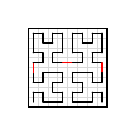
\begin{tikzpicture}
\tikzstyle{helperline} = [lightgray!60!white, line width=0.1mm];
\draw[line cap=round][helperline] (-0.0,0.125) -- (1.0,0.125);
\draw[line cap=round][helperline] (-0.0,0.25) -- (1.0,0.25);
\draw[line cap=round][helperline] (-0.0,0.375) -- (1.0,0.375);
\draw[line cap=round][helperline] (-0.0,0.5) -- (1.0,0.5);
\draw[line cap=round][helperline] (-0.0,0.625) -- (1.0,0.625);
\draw[line cap=round][helperline] (-0.0,0.75) -- (1.0,0.75);
\draw[line cap=round][helperline] (-0.0,0.875) -- (1.0,0.875);
\draw[line cap=round][helperline]  (0.125,1.0) -- (0.125,-0.0);
\draw[line cap=round][helperline]  (0.25,1.0) -- (0.25,-0.0);
\draw[line cap=round][helperline]  (0.375,1.0) -- (0.375,-0.0);
\draw[line cap=round][helperline]  (0.5,1.0) -- (0.5,-0.0);
\draw[line cap=round][helperline]  (0.625,1.0) -- (0.625,-0.0);
\draw[line cap=round][helperline]  (0.75,1.0) -- (0.75,-0.0);
\draw[line cap=round][helperline]  (0.875,1.0) -- (0.875,-0.0);
\draw[line cap=round]  (0,1) rectangle (1,0);
\draw[line cap=round] (0.0625, 0.0625) -- (0.0625, 0.1875);
\draw[line cap=round] (0.0625, 0.1875) -- (0.1875, 0.1875);
\draw[line cap=round] (0.1875, 0.1875) -- (0.1875, 0.0625);
\draw[line cap=round] (0.1875, 0.0625) -- (0.3125, 0.0625);
\draw[line cap=round] (0.3125, 0.0625) -- (0.4375, 0.0625);
\draw[line cap=round] (0.4375, 0.0625) -- (0.4375, 0.1875);
\draw[line cap=round] (0.4375, 0.1875) -- (0.3125, 0.1875);
\draw[line cap=round] (0.3125, 0.1875) -- (0.3125, 0.3125);
\draw[line cap=round] (0.3125, 0.3125) -- (0.4375, 0.3125);
\draw[line cap=round] (0.4375, 0.3125) -- (0.4375, 0.4375);
\draw[line cap=round] (0.4375, 0.4375) -- (0.3125, 0.4375);
\draw[line cap=round] (0.3125, 0.4375) -- (0.1875, 0.4375);
\draw[line cap=round] (0.1875, 0.4375) -- (0.1875, 0.3125);
\draw[line cap=round] (0.1875, 0.3125) -- (0.0625, 0.3125);
\draw[line cap=round] (0.0625, 0.3125) -- (0.0625, 0.4375);
\draw[line cap=round,red] (0.0625, 0.4375) -- (0.0625, 0.5625);
\draw[line cap=round] (0.0625, 0.5625) -- (0.1875, 0.5625);
\draw[line cap=round] (0.1875, 0.5625) -- (0.1875, 0.6875);
\draw[line cap=round] (0.1875, 0.6875) -- (0.0625, 0.6875);
\draw[line cap=round] (0.0625, 0.6875) -- (0.0625, 0.8125);
\draw[line cap=round] (0.0625, 0.8125) -- (0.0625, 0.9375);
\draw[line cap=round] (0.0625, 0.9375) -- (0.1875, 0.9375);
\draw[line cap=round] (0.1875, 0.9375) -- (0.1875, 0.8125);
\draw[line cap=round] (0.1875, 0.8125) -- (0.3125, 0.8125);
\draw[line cap=round] (0.3125, 0.8125) -- (0.3125, 0.9375);
\draw[line cap=round] (0.3125, 0.9375) -- (0.4375, 0.9375);
\draw[line cap=round] (0.4375, 0.9375) -- (0.4375, 0.8125);
\draw[line cap=round] (0.4375, 0.8125) -- (0.4375, 0.6875);
\draw[line cap=round] (0.4375, 0.6875) -- (0.3125, 0.6875);
\draw[line cap=round] (0.3125, 0.6875) -- (0.3125, 0.5625);
\draw[line cap=round] (0.3125, 0.5625) -- (0.4375, 0.5625);
\draw[line cap=round,red] (0.4375, 0.5625) -- (0.5625, 0.5625);
\draw[line cap=round] (0.5625, 0.5625) -- (0.6875, 0.5625);
\draw[line cap=round] (0.6875, 0.5625) -- (0.6875, 0.6875);
\draw[line cap=round] (0.6875, 0.6875) -- (0.5625, 0.6875);
\draw[line cap=round] (0.5625, 0.6875) -- (0.5625, 0.8125);
\draw[line cap=round] (0.5625, 0.8125) -- (0.5625, 0.9375);
\draw[line cap=round] (0.5625, 0.9375) -- (0.6875, 0.9375);
\draw[line cap=round] (0.6875, 0.9375) -- (0.6875, 0.8125);
\draw[line cap=round] (0.6875, 0.8125) -- (0.8125, 0.8125);
\draw[line cap=round] (0.8125, 0.8125) -- (0.8125, 0.9375);
\draw[line cap=round] (0.8125, 0.9375) -- (0.9375, 0.9375);
\draw[line cap=round] (0.9375, 0.9375) -- (0.9375, 0.8125);
\draw[line cap=round] (0.9375, 0.8125) -- (0.9375, 0.6875);
\draw[line cap=round] (0.9375, 0.6875) -- (0.8125, 0.6875);
\draw[line cap=round] (0.8125, 0.6875) -- (0.8125, 0.5625);
\draw[line cap=round] (0.8125, 0.5625) -- (0.9375, 0.5625);
\draw[line cap=round,red] (0.9375, 0.5625) -- (0.9375, 0.4375);
\draw[line cap=round] (0.9375, 0.4375) -- (0.9375, 0.3125);
\draw[line cap=round] (0.9375, 0.3125) -- (0.8125, 0.3125);
\draw[line cap=round] (0.8125, 0.3125) -- (0.8125, 0.4375);
\draw[line cap=round] (0.8125, 0.4375) -- (0.6875, 0.4375);
\draw[line cap=round] (0.6875, 0.4375) -- (0.5625, 0.4375);
\draw[line cap=round] (0.5625, 0.4375) -- (0.5625, 0.3125);
\draw[line cap=round] (0.5625, 0.3125) -- (0.6875, 0.3125);
\draw[line cap=round] (0.6875, 0.3125) -- (0.6875, 0.1875);
\draw[line cap=round] (0.6875, 0.1875) -- (0.5625, 0.1875);
\draw[line cap=round] (0.5625, 0.1875) -- (0.5625, 0.0625);
\draw[line cap=round] (0.5625, 0.0625) -- (0.6875, 0.0625);
\draw[line cap=round] (0.6875, 0.0625) -- (0.8125, 0.0625);
\draw[line cap=round] (0.8125, 0.0625) -- (0.8125, 0.1875);
\draw[line cap=round] (0.8125, 0.1875) -- (0.9375, 0.1875);
\draw[line cap=round] (0.9375, 0.1875) -- (0.9375, 0.0625);
\end{tikzpicture}
\end{document}

\section{The Proposed Method: GDDSG}\label{sec4}
\begin{figure*}
    \centering
    \includegraphics[width=\linewidth]{figures/framework.pdf}
    \caption{Illustration of The Overall Framework. [best view in color]}
    \label{fig: framework}
\end{figure*}
\textbf{Overview.} \autoref{fig: framework} provides an overview of our proposed method. 
Using task \( t \) as an example, we begin by projecting all training samples into an embedding space utilizing a pre-trained backbone. In this space, we compute the centroids for each class. Next, we evaluate whether a new centroid \( \mathbf{c}_i \) should be integrated into an existing class group \( G_j \).
If \( \mathbf{c}_i \) is dissimilar to all classes within \( G_j \), it is added to the group. If it is similar to any class in an existing group, it remains unassigned.
For unassigned centroids, we construct new similarity graphs (SimGraphs) based on their pairwise similarities. We then apply graph coloring theory to these SimGraphs, forming new class groups by clustering dissimilar categories together.
Finally, we update the NCM-based classifier with all class groups, facilitating efficient model updates with minimal computational overhead.

\subsection{Class Grouping Based on Similarity}

\autoref{Corollary: cor} provides guidance for constructing a sequence of dissimilar tasks. A key idea is to dynamically assign each new class to a group during CIL, ensuring that the similarity between the new class and other classes within the group is minimized. This approach helps maintain the robustness of each group's incremental learning process to the order of tasks. For each group, a separate adapter can be trained, and the results from different adapters can be merged during prediction to enhance the model's overall performance. 

In a given CIL task sequence, we organize the classes into several groups. The group list is denoted as \( G = [G_1, \dots, G_k] \), where each \( G_i \) represents a distinct group of classes. For a specified task \( t \) and each class \( C \in CLS^t \), our objective is to assign class \( C \) to an optimal group \( G^* \), ensuring that the new class is dissimilar to all existing classes in that group.

To achieve this objective, we first define the similarity between classes.
The similarity between any two classes, \( CLS_i \) and \( CLS_j \), is determined using an adaptive similarity threshold \( \eta_{i,j} \).
This threshold is computed based on the mean distance between the training samples of each class and their respective centroids in a learned embedding space, as shown below:

\begin{align}
    \eta_{i,j} = \max [
    & \frac{\sum_{k = 1}^{|X^t|} \mathbb{I}(y^t_k = i) \, d(h(x_k^t), \mathbf{c_i}) }{\sum_{k = 1}^{|X^t|} \mathbb{I}(y^t_k = i)}, \nonumber \\
    & \frac{\sum_{k = 1}^{|X^t|} \mathbb{I}(y^t_k = j) \, d(h(x_k^t), \mathbf{c_j}) }{\sum_{k = 1}^{|X^t|} \mathbb{I}(y^t_k = j)} 
    ],
\end{align}
where \( \mathbf{x}^{(t)} \) denotes the t-th task instance, \( h(\cdot) \) is the feature extraction function defined in Equation \autoref{eq: feature}, \( d: \mathcal{X} \times \mathcal{X} \to \mathbb{R}^+ \) specifies the distance metric space, \( \mathbb{I}(\cdot) \) represents the characteristic function, and the class centroid \( \mathbf{c}_i \in \mathbb{R}^d \) is computed as \( \mathbf{c}_i = \frac{1}{|C_i|} \sum_{x_j \in C_i} \mathbf{x}_j \).


Building upon this framework, we define the condition under which two classes, \( CLS_i \) and \( CLS_j \), are considered dissimilar. Specifically, they are deemed dissimilar if the following condition holds:

\begin{equation}
    d(\mathbf{c_i}, \mathbf{c_j}) > \eta_{i,j}.
    \label{eq: sim}
\end{equation}

Thus, class \( C \) is assigned to group \( G^* \) only if it is dissimilar to all classes within \( G^* \), and \( G^* \) is the choice with the lowest average similarity:

\begin{equation}
    G^* = \arg\min_{G} \frac{1}{|G|} \sum_{C' \in G} d(C, C').
\end{equation}

This approach is consistent with the principles outlined in \autoref{Corollary: cor} and ensures the robustness of the model across the entire task sequence.


\subsection{Graph-Driven Class Grouping}

Graph algorithms provide an efficient method for dynamically grouping classes while minimizing intra-group similarity.
In a graph-theoretic framework, classes are represented as nodes, with edge weights quantifying the similarity between them.
The flexibility and analytical power of graph structures allow for dynamic adjustment of class assignments in CIL, facilitating optimal grouping in polynomial time.
This approach significantly enhances the model's robustness and adaptability in incremental learning tasks.

Therefore, we can leverage the similarity between classes to construct a SimGraph, defined as follows:
\begin{definition} \textbf{(SimGraph.)}
A SimGraph can be defined as an undirect graph $SimG = (V, E)$, where $V$ is the set of nodes that represent each class's centroid and $E$ is the set of edges connecting pair of nodes that represent classes that are determined as similar by \autoref{eq: sim}.
\label{SimGraph}
\end{definition}

Then, we aim to partition the vertex set of this graph into subsets, with each subset forming a maximal subgraph with no edges between vertices. This problem can be abstracted as the classic NP-hard combinatorial optimization problem of finding a minimum coloring of the graphs. Let $G^{-1}(\cdot)$ be an assignment of class group identities to each vertex of a graph such that no edge connects two identically labeled vertices (i.e. $G^{-1}(i) \neq G^{-1}(j)$ for all $(i,j) \in E$). We can formulate the minimum coloring for graph $SimG$ as follows:
\begin{equation}
    \mathcal{X}(SimG) = \min | \{ G^{-1}(k) | k \in V\} |, 
    \label{eq: graph}
\end{equation}
where $\mathcal{X}(SimG)$ is called the chromatic number of $SimG$ and $|\cdot|$ denotes the size of the set.

Brooks' theorem \cite{brooks1941colouring} offers an upper bound for the graph coloring problem. To apply this in our context, we must demonstrate that the similarity graphs constructed in CIL meet the conditions required by Brooks' theorem. By doing so, we can establish that the problem is solvable and that the solution converges, ensuring the effectiveness of our grouping and class coloring process in class incremental learning. Without loss of generality, we can make the following assumptions:

\begin{assumption} In the CIL task, class \( C_i \) is randomly sampled without replacement from the set \( \mathcal{U} = \bigcup_{i=1}^{\infty} C_i \), ensuring that \( C_i \neq C_j \) for all \( i \neq j \). The probability that any two classes \( C_i \) and \( C_j \) within the set \( \mathcal{U} \) meet the similarity condition (as described in \autoref{eq: sim}) is denoted by \( p \).
\end{assumption}

In the CIL scenario with \( N \) classes, the probability of forming an odd cycle is given by \(\left( p^2(1-p)^{(N-2)} \right)^N = p^{2N}(1-p)^{N^2-2N}\). Similarly, the probability of forming a complete graph is \(p^{\binom{N}{2}} = p^{\frac{1}{2}N(N-1)}\).
Thus, the probability that the CIL scenario satisfies Brooks' theorem can be expressed as:
\begin{equation}
    P_{\text{Satisfy Brooks}'} = 1 - p^{2N}(1-p)^{N^2-2N} - p^{\frac{1}{2}N(N-1)}.
\end{equation}
\begin{figure}[t]
    \centering
    \includegraphics[width=\linewidth]{figures/contour_plot.pdf}
    \caption{Contour plot delineating the subthreshold region where \( P_{\text{Satisfy Brooks}'} < 0.99 \). The horizontal axis spans \( p \in [0.9, 1.0] \), representing probability values, while the vertical axis specifies sample sizes \( N \in [10, 40] \). In regions not displayed, the corresponding \( P_{\text{Satisfy Brooks}'} \) values exceed 0.99.}
    \label{fig: probability}
\end{figure}

\autoref{fig: probability} illustrates the various values of \( N \) and \( p \) that satisfy Brooks' theorem with a probability of less than 0.99. Our findings indicate that when \( N > 35 \), the CIL scenario adheres to Brooks' theorem. Furthermore, even with fewer classes, as long as \( p \) does not exceed 0.9, the CIL scenario can still ensure that the similarity graph complies with Brooks' theorem at a confidence level of 0.99. We conclude that class grouping based on the similarity graph is convergent and can be solved efficiently in polynomial time.

For \autoref{eq: graph}, while no algorithm exists that can compute \(\mathcal{X}(SimG)\) in polynomial time for all cases, efficient algorithms have been developed that can handle most problems involving small to medium-sized graphs, particularly the similarity graph \(SimG\) discussed here. In practical scenarios, such graphs are typically sparse. Notably, in conjunction with the above analysis, the similarity graph \(SimG\) in the CIL scenario satisfies the non-odd cycle assumption in Brooks' theorem \cite{brooks1941colouring}. For non-complete similarity graphs \(SimG\), we have \(\mathcal{X}(SimG) \le \Delta(SimG)\), where \(\Delta(SimG)\) represents the maximum vertex degree in \(SimG\).

Therefore, we can apply a simple yet effective greedy method, the Welsh-Powell graph coloring algorithm \cite{welsh1967upper}. This algorithm first sorts all nodes in the graph in descending order based on their degree and then assigns a color to each node, prioritizing those with higher degrees. During the coloring process, the algorithm selects the minimum available color for each node that differs from its neighbors, creating new color classes when necessary. The time complexity of this algorithm is \( O(|V|^2) \), primarily due to the color conflict check between each node and its neighbors. In theory, the maximum number of groupings produced by this algorithm is \( \max_{i = 1}^n \min\{ \deg(v_i') + 1, i \} \), with an error margin of no more than 1, where \( V' \) is the sequence of nodes sorted by degree, derived from \( V \).

\subsection{Overall Process}

\noindent \textbf{Training Pipeline.}
Building upon the theoretical foundations in Section 3.1, we now formalize the complete training procedure. Our framework leverages a frozen pre-trained feature extractor $\phi(\cdot)$, augmented with trainable random projections $W \in \mathbb{R}^{L \times M}$ where $M \gg L$, to enhance representation capacity. For each input $x_i^t$ from class group $s$, we compute its expanded feature:
\begin{equation}
\label{eq: feature}
h(x_i^t) = g(\phi(x_i^t) W) \in \mathbb{R}^M,
\end{equation}
where $g(\cdot)$ denotes the nonlinear activation.

The core learning paradigm reframes classification as regularized least-squares regression. Let $H_s^t \in \mathbb{R}^{N_s^t \times M}$ be the feature matrix and $Y_s^t \in \mathbb{R}^{N_s^t \times L_s^t}$ denote the one-hot label matrix for class group $s$. We optimize the projection matrix $\Theta_s^t \in \mathbb{R}^{M \times L_s^t}$ through:
\begin{equation}
\label{eq: loss}
\min_{\Theta} \|Y_s^t - H_s^t \Theta_s^t\|_F^2 + \lambda \|\Theta_s^t\|_F^2,
\end{equation}
where $\lambda$ controls regularization strength. The closed-form solution is:
\begin{equation}
\label{eq: analytic}
\Theta_s^t = ( {H_s^t}^\top H_s^t + \lambda I )^{-1} {H_s^t}^\top Y_s^t.
\end{equation}

For incremental updates, we maintain two key components: the Gram matrix $Gram_s^t$ capturing feature correlations, and the prototype matrix $C_s^t$ encoding class centroids. When new task $t$ arrives with $N_s^t$ samples:
\begin{equation}
    \label{eq: gram}
    Gram_{s}^t = Gram_{s}^{t-1} + \sum_{n = 1}^{N_{s}^t} h(x^t_i)^\top h(x^t_i),
\end{equation}
\begin{equation}
    \label{eq: pro}
    C_{s}^t = \begin{bmatrix}C_{s}^{t-1} & \underbrace{\mathbf{0}_M \ \mathbf{0}_M \ \ldots \ \mathbf{0}_M}_{(L_{s}^t - L_s^{t-1})\text{ times}} \end{bmatrix} + \sum_{n = 1}^{N_s^t} h(x^t_i)^\top y(x^t_i).
\end{equation}

The regularization parameter $\lambda$ is adaptively selected from a candidate pool $\Lambda$ through cross-validation on a held-out calibration set, minimizing the empirical risk:
\begin{equation}
\lambda^* = \arg \min_{\lambda \in \Lambda} \|Y_{\text{val}} - H_{\text{val}} (Gram_{\text{val}} + \lambda I)^{-1} C_{\text{val}} \|_F^2.
\end{equation}

Additionally, group descriptors are constructed through prototype similarity analysis. For each training instance $(x, y) \in \mathcal{D}^t$, we generate meta-features dataset as:
\begin{equation}
\mathcal{D}_g = \left\{ \left( \rho(x),\ G^{-1}(y) \right) \right\}_{(x,y)\in \mathcal{D}^t},
\end{equation}
where $\rho(x) = \big[ d(h(x),\mathbf{c}_1), \ldots, d(h(x),\mathbf{c}_k) \big]^\top$ denotes the concatenated distance vector measuring similarity between the sample embedding and prototype vectors.

\noindent \textbf{Inference Pipeline.}
Given test sample $x^*$, its group identification can be learned via $\hat{g} = \mathcal{M}_g(\rho(x^*))$, where $\mathcal{M}_g$ is the class group predict model trained with $ \mathcal{D}_g$.
Then, the prediction will be performed within the selected group via $\hat{y} = \underset{c \in \mathcal{C}_{\hat{g}}}{\arg\max}\ ( g(\phi(x^*) W) (Gram_{\hat{g}} + \lambda I)^{-1} C_{\hat{g}}[:,c]$.
        
\iffalse
In the previous section, we introduced the motivation and core concepts behind the proposed algorithm. In this section, we will describe the entire training process in detail. Recent years have seen CIL methods based on pre-trained models achieve remarkable results \cite{panos2023first,zhou2023revisiting,zhou2023revisiting,mcdonnell2024ranpac}, largely due to their robust representation capabilities. Since our proposed class grouping method also relies heavily on the model's representation ability, we utilize a widely-adopted pre-trained model as a feature extractor. For each class group, we train independent classification heads, which enhances the model’s adaptability and generalization to different class groups.

As outlined above, we utilize a frozen random projection matrix \( W \in \mathbb{R}^{L \times M} \) to enhance features across all class groups, where \( L \) is the output dimension of the pre-trained model and \( M \gg L \) is the expanded dimensionality. Given a task \( t \) and a sample \( x^t_i \) belonging to a class group \( s \), the feature vector of the sample is denoted as \( h(x^t_i) \), and its one-hot encoded label as \( y(x^t_i) \). Specifically,

\begin{equation}
    \label{eq: feature}
    h(x^t_i) = g(\phi(x)^T W),
\end{equation}
where \( \phi(\cdot) \) represents the feature extractor, and \( g(\cdot) \) is a nonlinear activation function.
We define \( H_{s}^t \in \mathbb{R}^{N_{s}^t \times M} \) as the matrix containing feature vectors of \( N_{s}^t \) samples from group \( s \). The corresponding Gram matrix is defined as:
\begin{equation}
    \label{eq: grammatrix}
    Gram_{s}^t = {H_{s}^t}^T H_{s}^t \in \mathbb{R}^{M \times M}.
\end{equation}
Additionally, the matrix \( C_{s}^t \) consists of the concatenated column vectors of all classes within group \( s \), with dimensions \( M \times L_{s}^t \), where \( L_s^t \) represents the number of classes in group \( s \) for task \( t \). When a new task arrives, the model applies the GDDSG algorithm to assign new classes to their respective groups. The Gram matrix \( Gram \) and matrix \( C \) for each group are updated according to the following formulas:
\begin{equation}
    \label{eq: gram}
    Gram_{s}^t = Gram_{s}^{t-1} + \sum_{n = 1}^{N_{s}^t} h(x^t_i) \otimes h(x^t_i),
\end{equation}
\begin{equation}
    \label{eq: pro}
    C_{s}^t = \begin{bmatrix}C_{s}^{t-1} & \underbrace{\mathbf{0}_M \ \mathbf{0}_M \ \ldots \ \mathbf{0}_M}_{(L_{s}^t - L_s^{t-1})\text{ times}} \end{bmatrix} + \sum_{n = 1}^{N_s^t} h(x^t_i) \otimes y(x^t_i),
\end{equation}
where \( \mathbf{0}_M \) denotes a zero vector with \( M \) dimensions.

During the test phase, we combine the classification heads of all groups \( G = [G_1, G_2, \dots, G_k] \) to make a joint prediction for a given sample \( x \). For each class \( c' \) in a group, the score is computed as follows:
\begin{equation}
    \label{eq: predict}
    s_{c'} = g(\phi(x)^T W)(Gram_{i} + \lambda I)^{-1} C_{c'},
\end{equation}
where \( i = 1,\dots,k \) denotes the indices of each groups, and \( \lambda \) is the regularization parameter used to ensure that the \( Gram \) matrix remains invertible. The final classification result is then obtained by applying the following formula:
\begin{equation}
    \label{eq: predict_joint}
    \hat{c} = \mathop{\arg\max}\limits_{c' \in \cup_{i = 1}^k CLS^{G_i}} s_{c'},
\end{equation}
where \( \cup_{i = 1}^k CLS^{G_i} \) represents the set of possible classes across all class groups.
\fi

\section{Perspectives}

\subsection{MADRL Should Leverage Direct Interpretability}

Engaging and expanding interpretability is an opportunity to address existing challenges in MADRL. Direct approaches are particularly well-suited for analysing communication dynamics, coordination strategies, and emergent behaviours in MAS. Graph-based analysis, for instance, could provide insights into inter-agent interactions, while feature importance techniques can identify biases and ensure fairness in decision-making. By systematically exploring and applying scalable direct methods to trained models, researchers can better address the inherent complexities of MADRL, enabling the development of more transparent, robust, and accountable systems for real-world applications.

Although previous calls to action are prone to integrate interpretability beforehand \cite{rodriguez2024explainable}, this paper claims that the interpretation of models post hoc is highly valuable. Direct interpretability offers greater flexibility, particularly for existing models where architectural modifications are impractical. 

\subsection{Robust Evaluation Protocols}

As repeatedly outlined, direct post-hoc methods are easily actionable and scalable.
However, their adoption requires acknowledging and addressing limitations such as the inherent shortcomings of saliency maps \cite{Adebayo2018SanityCF,Bilodeau2022ImpossibilityTF}, counterfactual explanations \cite{Laugel2019TheDO}, or other interpretability illusions \cite{Bolukbasi2021AnII,Friedman2023InterpretabilityII,Friedman2023InterpretabilityII}. In fact, these methods often generate metrics with limited predictive power, and thus, claims should be reasonable.


A key priority is the development of robust evaluation protocols for direct methods. Given the absence of ground-truth explanations, reliable metrics and standardized evaluation frameworks must be established to assess the quality and utility of these methods \cite{Gill2020ARM,Madsen2021PosthocIF,Amorim2023EvaluatingPI,Hedstrm2022QuantusAE,Wei2024RevisitingTR,Huang2024RAVELEI,Chaudhary2024EvaluatingOS}. 
Advancing evaluation thoroughly, e.g., by evaluating out of distribution, is especially important to develop scalable, effective, and actionable interpretability solutions.


\section{Conclusion}

We outlined that direct interpretability might be vital for addressing the challenges of scalability and complexity in modern MADRL. It enables the analysis of trained models without imposing architectural constraints, providing critical insights into agent behaviour, emergent dynamics, and biases. Advancing these methods will ensure scalable oversight of these systems, which is a precious desideratum for real-world applications. However, challenges such as explanation illusions, lack of robust evaluation metrics, and difficulty disentangling causal effects should be considered and tackled.



%%%%%%%%%%%%%%%%%%%%%%%%%%%%%%%%%%%%%%%%%%%%%%%%%%%%%%%%%%%%%%%%%%%%%%%%

%%% The next two lines define, first, the bibliography style to be 
%%% applied, and, second, the bibliography file to be used.

\bibliographystyle{ACM-Reference-Format} 
\bibliography{main}

%%%%%%%%%%%%%%%%%%%%%%%%%%%%%%%%%%%%%%%%%%%%%%%%%%%%%%%%%%%%%%%%%%%%%%%%

\end{document}

%%%%%%%%%%%%%%%%%%%%%%%%%%%%%%%%%%%%%%%%%%%%%%%%%%%%%%%%%%%%%%%%%%%%%%%%

